\documentclass{boi2014-de}

\usepackage{enumitem}

\renewcommand{\DayNum}{2}
\renewcommand{\TaskCode}{postmen}
\renewcommand{\TaskName}{Seniorenbriefträger}
\renewcommand{\TaskVersion}{1.1}

\begin{document}
    \begin{wrapfigure}[8]{r}{4cm}
        \vspace{-18pt}
		\includegraphics[width=4cm]{\TaskCode.jpeg}
	\end{wrapfigure}
    Wir schreiben das Jahr 2036 und Europa ist voll von Senioren. Um sie bei Gesundheit zu halten, plant das Ministerium für den Schutz von Mehrheiten, sie die kleine Menge Papierpost austragen zu lassen, die noch verschickt wird --- typischerweise an Senioren. Dieser Plan wird in ganz Europa umgesetzt.
    
    Das Ministerium hat folgendes ``Seniorenpostsystem'' erdacht: Europa wurde in Bereiche eingeteilt, wobei jeder Bereich aus einer Menge von Kreuzungen und Straßen, die diese Kreuzungen miteinander verbinden, besteht. Jede Straße kann in beiden Richtungen begangen werden. In jedem Bereich können beliebig viele Senioren als Briefträger angeheuert werden. Jeden Morgen bekommt jeder Briefträger eine Tasche mit Briefen, die er auf einem Weg im Straßennetz seines Bereichs abliefern soll. Jeder Weg muss dabei \emph{seniorenkompatibel} sein, das heißt:

    \begin{itemize}
        \item Er startet und endet an derselben Kreuzung.
        \item Er führt nicht mehrfach über dieselbe Kreuzung (um die Senioren nicht zu verwirren).
        \item Keine Straße darf von mehr als einem Briefträger begangen werden (um Schlägereien zwischen den Senioren vorzubeugen).
    \end{itemize}
    
    Alle Wege zusammen sollen das gesamte Netzwerk abdecken: Das heißt, dass jede Straße von genau einem Briefträger beliefert wird.

    \Task
    Das Ministerium benötigt ein Computerprogramm, das für ein gegebenes Straßennetz eine solche Menge von seniorenkompatiblen Wegen berechnet.

    \Input
    Die Eingabe beschreibt das Straßennetz.
  
    Die erste Zeile enthält zwei ganze Zahlen $N$ und $M$.
    $N$ ist die Anzahl der Kreuzungen und $M$ die Anzahl der Straßen.
    Kreuzungen sind von $1$ bis $N$ nummeriert.
  
    Jede der folgenden $M$ Zeilen enthält zwei ganze Zahlen $u$ und $v$
    ($1 \le u, v \le N, u \neq v$), die anzeigen, dass es eine Straße zwischen den Kreuzungen $u$ und $v$ gibt.

    Für alle Eingabedaten gilt:
    \begin{enumerate}
        \item Zwei Kreuzungen sind durch höchstens eine Straße direkt miteinander verbunden.
        \item Jede Kreuzung kann von jeder anderen Kreuzung erreicht werden (ggf. über Zwischenpunkte).
        \item Es gibt eine Lösung --- also eine Menge von seniorenkompatiblen Wegen, die das Straßennetz komplett abdecken.
    \end{enumerate}

    \Output
    Jede Zeile der Ausgabe soll einen seniorenkompatiblen Weg beschreiben.
    Ein Weg wird beschrieben durch die Nummern der Kreuzungen, über die er führt in der Reihenfolge, in der sie passiert werden.
    Der Startpunkt (der auch der Endpunkt ist) soll dabei als erstes Ausgegeben werden und nur einmal.
    
    Falls mehr als eine Lösung existiert, kannst du eine beliebige ausgeben.

    \Example

    \example
    {
        10 15 \newline
        1 3 \newline
        5 1\newline
        2 3 \newline
        9 2\newline
        3 4 \newline
        6 3\newline
        4 5 \newline
        7 4\newline
        4 8 \newline
        5 7 \newline
        8 5\newline
        6 7 \newline
        7 8 \newline
        8 10 \newline
        10 9
    }
    {
        2 3 4 5 8 10 9 \newline
        7 8 4 \newline
        1 5 7 6 3
    }
    {
        Das folgende Bild illustriert das Straßennetz und die drei seniorenkompatiblen Wege, die verwendet werden könnten, um es abzudecken.

        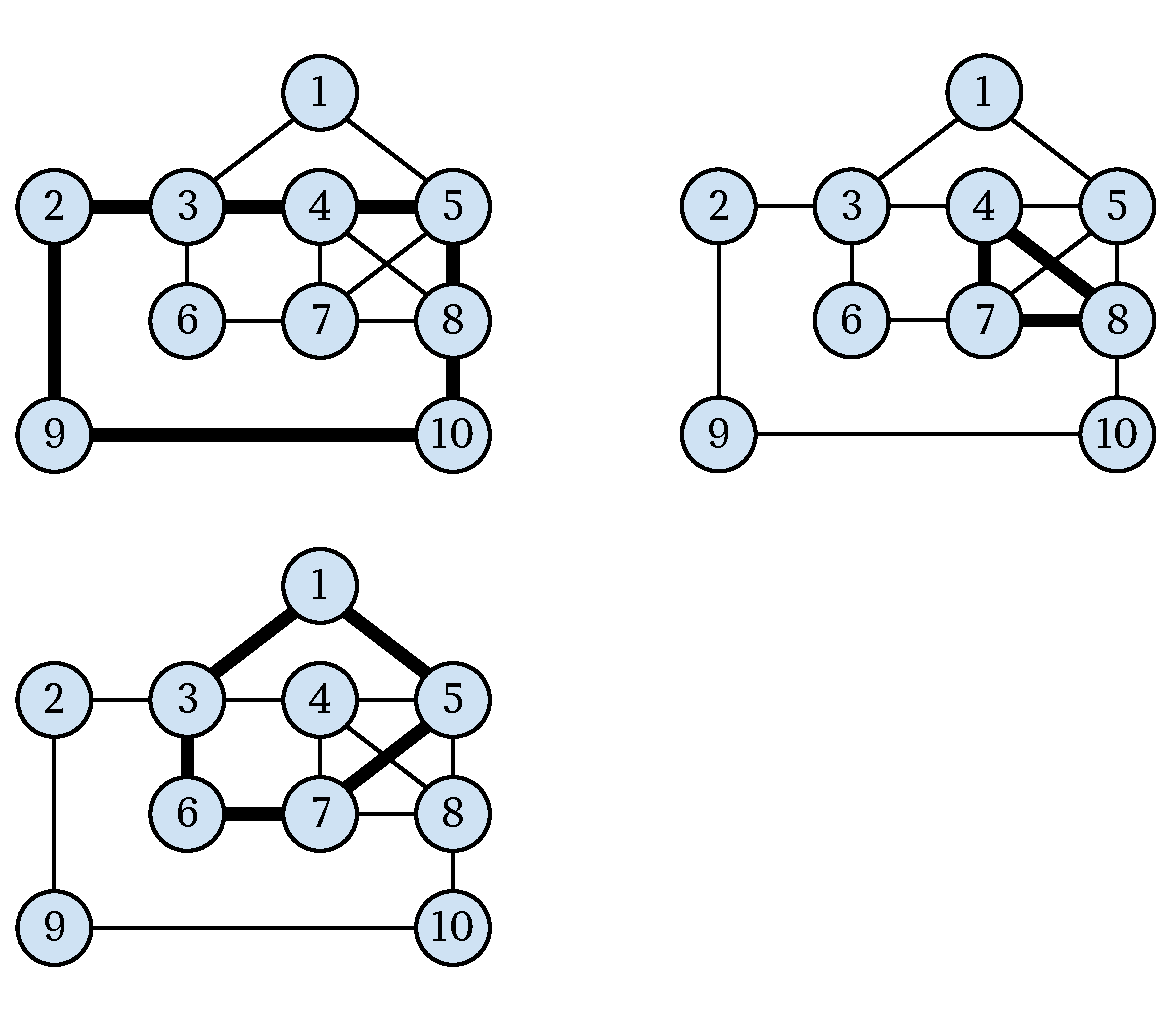
\includegraphics[width=7cm]{senior-example}

        Bemerke, dass es in diesem Beispiel mehrere Lösungen gibt, auch welche, die nur zwei Wege benötigen.    
    }

    \Scoring

    \begin{description}
        \item[Teilaufgabe 1 (38 Punkte):] $3 \le N \le 2\ 000$, $3 \le M \le 100\ 000$.
        \item[Teilaufgabe 2 (17 Punkte):] $3 \le N \le 100\ 000$, $3 \le M \le 100\ 000$.
        \item[Teilaufgabe 3 (45 Punkte):] $3 \le N \le 500\ 000$, $3 \le M \le 500\ 000$.
    \end{description}

    \Constraints

    \begin{description}
        \item[Zeitlimit:] 0.5 s.
        \item[Speicherlimit:] 256 MB.
    \end{description}

\end{document}
